\documentclass[twocolumn]{article}
\usepackage[top=1.1in, left=0.85in, right=0.85in]{geometry}

\usepackage{amsmath}
\usepackage{amssymb}
\usepackage{code}
\usepackage{graphicx}

\pagestyle{empty}

\newcommand[1]{comment}{}
\newcommand[1]{parameteralert}{
  % XXX this can get cooler.
  {\bf Parameter Alert!}\,\, #1
}

% XXX superscript
\newcommand\th{th}

% \usepackage{ulem}
% go back to italics for emphasis, though
% \normalem

\begin{document} 

\title{The First Level of Super Mario Bros.~is Easy with
       Lexicographic Orderings and Time Travel
       {\normalsize \ldots after that it gets a little tricky.}}
\author{Dr.~Tom~Murphy~VII~Ph.D.\thanks{
Copyright \copyright\ 2013 the Regents of the Wikiplia
Foundation. Appears in SIGBOVIK 2013 with the reluctant sigh of the
Association for Computational Heresy; {\em IEEEEEE!} press,
Verlag-Verlag volume no.~0x40-2A.
CHF 0.00}
}


\renewcommand\>{$>$}
\newcommand\<{$<$}

\date{1 April 2013}

\maketitle

\begin{abstract}
This is where the Abstract goes.
\end{abstract}

\vspace{1em}
{\noindent \small {\bf Keywords}:
  computational super mario brothers, memory inspection, lexicographic induction, networked entertainment systems, pit-jumping, ...

}

\section*{Introduction}
The Nintendo Entertainment System is probably the best video game console, citation {\it not} needed. Like many, I have spent thousands of hours of my life playing NES games, including several complete playthroughs of classics like Super Mario Bros., Bionic Commando, Bubble Bobble, and other favorites. By the year 2013, home computers have become many orders of magnitude faster and more capacious than the NES hardware. This suggested to me that it may be time to automate the playing of NES games, in order to save time.\footnote{Rather, to replace it with time spent programming.} In this paper I present a generic technique for automating the playing of NES games. The approach is practical on a single computer, and succeeds on some games, such as Super Mario Bros.. The approach is amusingly elegant and surprisingly effective, requires no detailed knowledge of the game being played, and is capable of novel and impressive gameplay (for example, bug exploitation). {\bf Disclaimer for SIGBOVIK audience: This work is 100\% real.}

On a scale from ``the title starts with Toward'' to ``Donald Knuth has finally finished the 8\th\ volume on the subject'', this work is a 3. The purpose of this paper is mainly as a careful record of the current status for repeatability and further development on this important research subject. A short video version of this paper is available for those that hate reading, at \verb+http://tom7.org/mario+, and is the more fun way to consume the results. This page also contains audiovisual material that makes this work more entertaining (for example, its output) and source code.

The basic idea is to deduce an objective function from a short recording of a player's inputs to the game. The objective function is then used to guide search over possible inputs, using an emulator. This allows the player's notion of progress to be generalized in order to produce novel gameplay. A design goal is that the objective function be amusingly elegant (not at all smart, fancy, or customized to the game) in order to demonstrate that the game is reducible to such a simple objective. The search needs to be game-agnostic and practical, but since the space is exponential ($256^{n}$), we need to be smart here.

The objective function, the algorithm to deduce it, the search strategy, and its implementation are all interesting and will be discussed in that order. To set the stage, I begin with a description of the NES hardware and emulation of it.

\subsection{The NES hardware and emulation}
The NES is based around an 8-bit processor running at 1.79~MHz, the Ricoh 2A03. 8 bits is really small. You can see them all right here: 00001111. It's no coincidence that each controller also has 8 buttons: Up, Down, Left, Right, Select, Start, B and A. It has only 2048 bytes of general purpose RAM. (There is also some special purpose RAM for graphics, which we ignore in this work.) 2048 bytes is really small. You can see them all in Figure~\ref{fig:bytes2048}. As a result, NES programs are written to use memory efficiently and straightforwardly; usually there are fixed memory locations used for all the critical game facts like the player's health, number of lives, coordinates on the screen, and so on. For example, in Super Mario Bros., the single byte at location \verb+0x757+ contains the number of lives the player has. The location \verb+0x75F+ contains the current world, and \verb+0x760+ the current level.

% (32kB of ROM is addressable at a time, and most games used bank switching to access hundreds of kilobytes of game included in the cartridge.) 

There are a number of emulators for NES. These work by simulating the NES hardware, for example with a 2048-byte array for its memory, and simulating the steps of its 2A03 processor on some ROM, and hooking a keyboard or joystick into the 8 bits of input. (There are of course many details to work out! But in essence emulation is jut that.) This process is completely deterministic, so it is possible to record the sequence of inputs (the inputs can only be read once per video frame, so this sequence is 60 \comment{ XXX CHECK } bytes per second) and play them back and get the same result. This also means that an input sequence can be computed in non-real time, either much slower or much faster than a NES would normally run. In this work we use the FCEUX emulator, which is popular for its accuracy and advanced tools.

\begin{figure}
\begin{center}
% XXX make image
% 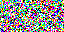
\includegraphics[width=0.75 \linewidth]{bytes2048}
\end{center}\vspace{-0.1in}
\caption{2048 bytes, a 64x32 image.}
\label{fig:bytes2048}
\end{figure}

\section{Objective function}

Bytes in memory (and sometimes 16- and 32-bit words) can contain interesting game facts like the player's position in the level or score. The central idea of this paper is to use (only) the value of memory locations to deduce when the player is ``winning''. The things that a human player perceives, like the video screen and sound effects, are completely ignored. As an additional simplification, we assume that winning always consists of a value {\it going up}---either the position in the level getting larger, the score getting larger, the number of lives, the world or level number getting bigger, etc.

This is actually a little bit too naive; for example, Mario's overall progress through the game is represented by a pair. You start in World 1-1 and the underground level that comes next is World 1-2 (we'll call this $w=1$ and $\ell=2$). But after you discover the princess is in another castle in World 1-4, the next level is 2-1.\footnote{In case you never realized this, it is time to learn that the legendary ``Minus World'' of \verb+ -1+ is not actually a negative world, but World 36-1 being incorrectly rendered because there is no glyph for the 36\th\ digit. The trick used to get to the Minus World just happens to leave the value 36 in that memory location rather than initializing it to a useful value. The ROM does not contain data for world 36 so it just interprets garbage data as a description of the world.} This can't be represented as a single byte going up (sometimes the second part $\ell$ goes down when we get to a new first part $w$), but it can be represented as a lexicographic order on the pair $\langle w, \ell \rangle$; that is, $\langle w_1, \ell_1 \rangle < \langle \w_2, \ell_2$ if $\w_1 = \w_2$ and $\ell_1 < \ell_2$, or if $\w_1 < \w_2$ no matter the values of $\ell_1$ and $\ell_2$. This matches our intuitive idea and is also mathematically nice. It also generalizes multi-byte encodings of things like your score (which can be larger than 8 bits and so is often stored in 16 or 32), including both big-endian and little-endian representations.\footnote{A possible additional simplification would be to just take lexicographic orderings over bits, which then generalizes to 8-bit bytes. This is probably too crazy, but just right now I am sort of feeling like maybe I should try it, though it may be the beer.}

More importantly, it allows the combination of semantically unrelated bytes, like: $\langle$ world, level, screen inside the world, $x$ position on the screen $\rangle$ or $\langle$ world, lives, low byte of score $\rangle$. Many orderings may describe gameplay. These orderings may be temporarily violated in normal play: Although the score always goes up, Mario's $x$ position may temporarily decrease if he needs to navigate around some obstacle.\footnote{Note to self: Maybe we should give a much higher score to globally preserved objectives than to locally preserved ones. But that may presuppose that the input represents a whole playthrough?} So, to ``faithfully'' represent gameplay, we will generate a set of lexicographic orderings on memory locations, with the idea that they ``generally go up'' but not necessarily at every step. These orderings will also have weights. The next section describes how we take a sequence of player inputs and deduce the orderings.

\subsection{Deriving the objective function} \label{sec:deriving}

In order to derive an objective function, we'll start with an abstract
subroutine that finds a single lexicographic ordering
nondeterministically. This function takes in an ordered list of $n$
memories $M_1\ldots M_n$ which all have size $m$ bytes. For example,
$m = 2048$ and $n = 100$, for the memories at each of the first $100$
frames of someone playing Super Mario Bros.. It produces an ordered
list of unique memory locations $L_1 \ldots L_k$ (where $0 \leq L_i <
m$, that is, each is some spot in the 2048 bytes of RAM) that is a
{\em maximal} {\em tight} {\em valid} lexicographic ordering of $M$.
Let's start by defining those terms just to be careful.

Given some list of memory locations $L_1 \ldots L_k$ and a pair of
memories $M_a$ and $M_b$, we say that $M_a =_L M_b$ iff $M_a[L_1] =
M_b[L_1]$ and $M_a[L_2] = M_b[L_2]$ and so on for every $L_i$; that
is, the bytes must be equal at each of the locations. Easy. We say
that $M_a <_L M_b$ iff there exists some $p \leq k$ where $M_a[L_1] =
M_b[L_1] \ldots M_a[L_{p-1}] = M_b[L_{p-1}]$ and $M_a[L_p] <
M_b[L_p]$. Put simply, if the two memories are not equal according to
$L$ (have the same byte at every memory location) then there is a
unique first location ($L_p$) where they have a different byte, and
that byte determines the order. $M_a >_L M_b$ is just defined as $M_b <_L
M_a$; $M_a \leq_L M_b$ is just $M_a <_L M_b$ or $M_a =_L M_b$, and similarly
for $\geq_L$, and they mean what you think so don't worry.

Every $L$ defines a lexicographic ordering ($<$ and $=$ operators).
$L$ is a {\em valid} lexicographic ordering of $M$ if $M_i \leq_L M_{i + 1}$
for $1 \leq i \leq n$; each memory is less than or equal to the next
memory in the sequence. It follows that $M_i \leq_L M_j$ whenever $i < j$.

Every prefix of a valid $L$ (including the empty prefix) is a valid
lexicographic ordering as well. On a scale from useless to useful, the
empty prefix is a 1 (it equates all memories), which suggests that
some orderings are better than other. To give a primitive notion of
``good'' lexicographic orderings, we define a {\em maximal} valid
lexicographic ordering to be $L$ such that there are no extensions of
$L$ that are valid. An extension of $L_1 \ldots L_k$ is just $L_1
\ldots L_k, L_{k+1}$ (where $L_{k+1} \neq L_i$ for $1 \leq i \leq k$):
Some new memory location that we put at the end of the order (in the
least important position). We do not consider extending in the middle
of the order or beginning, although that would make sense.

Maximal valid orderings are good and it is straightforward to produce
them (a less constrained version of the algorithm below), but they
have the bummer downside that memory locations that never change value
for any $M$ can be included at any position of the ordering, and all
such choices are equivalent. And in fact all locations {\em must} be
included to make the ordering {\em maximal}. This is bad because when
$M$ contains many locations with fixed values, we have boatloads of
equivalent orderings, and they're also longer than necessary. An {\em
  tight} valid ordering is one where for each $L_i$ there exists at
least one $M_a$ and $M_{a+1}$ where $M_a[L_i] < M_{a+1}[L_i]$ and
$M_a[L_j] = M_{a+1}[L_j]$ for all $i < j$; that is, every location has
to participate in the ordering at least once. The notion of {\em
  maximal} has to be relative to this property as well---a {\em tight
  extension} is one that produces a tight valid ordering, and a {\em
  maximal tight valid ordering} permits no tight extensions.

On a scale from simple to fancy, this algorithm is a 3. Given those
definitions, the idea is to start with the empty prefix, which is
always a tight valid lexicographic ordering but usually not maximal.
We then pick a tight extension that is valid; if none exists then we are
done and have a maximal tight valid ordering. Now we have a new tight valid
ordering, and we repeat.

The pseudocode gives a pseudoimplementation of the algorithm that is
more pseudodetailed. The C++ implementation is in \verb+objective.*+.
C++ is not a good language for this kind of program but we use it
because the NES emulator is written in C++.

\begin{figure}[htp]
  \begin{code}
    (* Prefix is the prefix so far (int list)
       and remain is the list of memory locations
       that we can still consider. Invt is that
       prefix is a tight valid ordering on M. Returns
       the memory locations from remain that are
       a tight extension of the prefix. *)
    fun candidates (prefix, remain) =
      let lequal = (* list of indices $i$ where
                      $M_i =_{\tt prefix} M_{i+1}$ *)
      let notgreater = (* members $x$ of remain where
                          $M_i[x] > M_{i + 1}[x]$ is
                          not true for any $i$ in
                          {\tt lequal} *)
      let tight = (* members $y$ of notgreater where
                     $M_i[x] < M_{i + 1}[x]$ is true
                     for some $i$ in {\tt lequal} *)
      in tight
                          
    (* Returns a maximal tight valid ordering, given
       a tight valid prefix and list of memory locations
       we are permitted to consider. *)
    fun ordering (prefix, remain) =
      case candidates (prefix, remain) of
        (* No extensions means it's maximal. *)
        nil => prefix
      | cand =>
        let c = nondeterministically-choose-one cand
        let remain' = remove-element (remain, c)
        let prefix' = prefix @ [c]
        in ordering (prefix', remain')
  \end{code}

  \caption{Pseudocodes for nondeterministically generating a maximal
    tight valid lexicographic ordering on some memories $M$. The
    recursive function {\tt ordering} just orchestrates the selection
    of an extension until there are no possibilities remaining, and
    returns it. The function {\tt candidates} finds all the possible
    extensions for a prefix. First we compute {\tt lequal}, all of the
    adjacent memory pairs (represented by the index of the first in
    the pair) where the memories are equal on the prefix. Only pairs
    that are equal on the prefix are interesting because these are the
    only ones that will even depend on the extension to the prefix
    when comparing the memories. We only need to consider adjacent
    pairs because on an a scale of exercise for the reader to proof is
    contained in the extended technical report, this statement is a
    you can figure that one out yourself. Valid extension locations
    are ones where the memory pairs are never increasing at that
    location (note that in places where pairs are not equal but
    strictly less on the prefix, it's perfectly fine for the extension
    to be greater; this is the ``point'' of lexicographic orderings).
    Finally, tight extensions are those valid ones that have at least
    one pair of memories where the location has a value that is
    strictly less.}
  \label{fig:ordering}
\end{figure}

\subsection{The objective function, in practice}

We can't just use a single objective function. Choosing objective
functions nondeterministically, we may get a crap one like ``High byte
of the score'' which only goes up once during all of our memory
observations. We also can't just use all of the memory observations,
because there may be brief moments that violate strict orderings, like
Mario's $x$ coordinate temporarily decreasing to navigate around an
obstacle. More starkly, the first few hundred frames of the game are
almost always initialization where the memory temporarily takes on
values that are not representative of later gameplay at all. In
practice, we use the nondeterministic function from
Section~\ref{sec:deriving} on multiple different slices of the memory
observations. We also call it many times to nondeterministically
generate many different objectives. Finally, we weight the objectives
by how representative we think they are.

\parameteralert{This one of the first places where we have some
  arbitrary constants, which are the enemy of elegance. On a scale of
  ballpark to obsessively overfit, these constants are a 2; I
  basically looked at some graphs while developing the objective
  function learning part of the code to decide whether they were
  ``good enough'' and didn't tune them after starting to observe
  actual performance. Some of those graphs appear in figures here.
  For all I know, these are really bad choices, but it was important
  for aesthetic reasons for the objective function to be brutish. The
  only reason to permit these parameters at all is that it simply
  does not work to have a single ordering or to use only orderings
  that apply to the whole memory.}

{\bf Skipping.}\,\, To avoid being confused by RAM initialization and
menu, I ignore all memories up until the first input by the player.
Including these would be especially suspicious because the RAM's
contents are not even well-defined until the program writes something
to them.\footnote{Emulators tend to fix them to a specific pattern so
  that emulation is completely deterministic, but in real hardware
  they are truly uninitialized, or retain the values from the last
  reset or game inserted. Some semi-famous tricks involve removing
  and inserting game cartridges while the system is running in order
  to take advantage of this.}

% XXXX good place for some graphs.
{\bf Slicing.}\,\, I generate 50 orderings for $M_1 \ldots M_n$; the
whole recording starting from the first keypress. During gameplay some
values really are completely nondecreasing, like the player's score
and world/level pair. I also generate 3 orderings for each tenth of
the memory sequence, e.g. $M_1 \ldots M_{n/10}$ and $M_{n/10+1} \ldots
M_{2n/10}$, etc. The intention is to capture orderings that are rarely
violated, or sections of the game with unusual objectives (e.g. a
minigame or swimming level). Orderings generated this way look pretty
random, and on a scale from solid to suspicious, I can't vouch for
them. Then I generate objectives from non-consecutive memories that
are evenly spread out through the observations: Ten objectives
chosen from every 100\th\ memory, starting from the 0\th\ frame,
1\st\ frame, 2\nd\ frame, and so on up to the 9\th{}. Similarly
for every 250\th\ frame, and a single objective for memory sliced
to every 1000\th\ frame, with start positions of 0--9.

{\bf Weighting.},\, To reduce the importance of randomness in the
learning process, and the arbitrariness of the slicing, each objective
function is also assigned a weight. An ideal objective function takes
on its minimal value on the first frame and maximal on the last
(according to the ordering), and increases steadily throughout the
observed memories. This is ideal because it allows us to just follow
the gradient to reach good states. A bad objective function freqently
regresses (recall that although we produce valid orderings, an
ordering that is valid on some slice may not be valid for the whole
sequence of memories). To weight an objective $L$, we first collect
all of the values (the vector of values of the memory locations $L_1
\ldots L_k$) it takes on throughout the observations. These may not
obey the ordering. We then sort the values lexicographically and
remove duplicates.\footnote{Note to self: I'm not sure how to justify
  removing duplicates here. It makes [0, 1, 1, 1, 1, 1, 10, 11] look
  the same as [0, 1, 10, 11], which is probably not desirable?} Call
this $V$. Now we can compute the {\em value fraction} for $L$ on some
$M$: Extract the vector of locations $M[L_1], M[L_2], \ldots, M[L_k]$
and find the lowest index $i$ in $V$ where the vector is less than or
equal to $V_i$. The value fraction {\tt VF} is $i/|V|$, which is the
normalized value of ``how big'' $M$ is, according to $L$, compared to
all the values we ever saw for it. The value fraction is defined and
in $[0, 1]$ for all memories in the observed set.\footnote{It is not
  defined when the memory is greater than all observed memories, which
  we will encounter later. The code returns $(i+1)/|V|$ in that case,
  which is as good as anything.} This gives us the ability to compare
objectives on an absolute scale.\footnote{This is certainly not the
  only way to do it, and it has some questionable properties like
  ignoring the magnitude of change. But it is very simple.} Weighting
an objective is now simple:
%
$$ \Sigma_{i=1}^{n-1}  {\tt VF}($M_{i+1}$) - {\tt VF}($M_{i}$) $$
%
We sum the differences in value functions for each consecutive pair of
memories. In the case of the ideal function this is \Sigma_{i=1}^{n-1}
$1/n$, which approaches $1$.\footnote{The code implements a different
  weighting scheme, which sums from $i=0$ and keeps track of the last
  value fraction at each step, thus treating the value fraction of the
  nonexistent memory $M_0$ as 0. This is wrong, because the first
  value fraction may be very high, which credits the objective with a
  positive value (e.g. 1) for that first part of the sum. Objectives
  that start high on the first frame are not ideal; in fact, the worst
  objectives start high on the first frame and steadily {\em
    decrease}. I plan to correct this bug and study if it has any
  noticeable consequences.} Objectives are constrained to have
non-negative weights (I set the value to 0 if negative, which
effectively disables it).

% XXX good place to give some weights for some objectives.

We save the objectives and their weights to a file and then we are
done with the easy part.

\subsection{Motifs} \label{sec:motifs}

The very first thing I tried with the objective function is to just do
some greedy search for input sequences that increased the objective.
This works terribly, because the search space for inputs is large
($2^8$ possibilities at each frame). Most are useless (it's almost
impossible to press the left and right directions at the same time,
and real players almost never do it); real input sequences usually do
not change values 60 times per second (rather, the player holds the
jump button for 10--20 frames); some button-presses and combinations
are much more common than others (e.g. right+B is common for running
right, but start pauses the game). Search quickly necessitates a model
for inputs. Rather than do anything custom, I just use a really dumb
approach: Take the observed inputs (the same ones that we learned the
objective functions from) and split them into chunks of 10 inputs.
Motifs are weighted by the number of times they occur in the input.
There may be a single motif at the end that's fewer than 10 inputs.

\parameteralert{Here I choose the magic number 10 for the size of input
  motifs. On a scale from gravitational constant to pulled it out of
  my ass, this is an 8. We could perhaps justify 10 as being close to
  the speed of input change actually possible for a human (6 button
  presses per second; 166ms). I believe it is possible to do much
  better here and the code contains a few such false starts, but using
  motifs was one of the biggest immediate improvements in the history
  of this code, so I went with it. A natural thing to try is a Markov
  model, although this has a free parameter too (the number of states
  of history). It is likely possible to do some kid of abstract
  interpretation where multiple different input sequences with
  equivalent outcomes are explored simultaneously, which might obviate
  the need for computing an input model from the observed play. The
  playfun algorithm below takes motifs as primitive because of the way
  it was developed; I'll use footnotes to describe my thinking about
  how to remove this.}

Motifs are written to a file too and then we're done with that. This
concludes the learning we do from the example input; everything else
is a matter of using the objective functions and motifs to play the
game.

\section{Now you're playing with power}

In this section I'll describe how the objective functions are used to
play the game. On a scale from canonical to Star Wars Christmas
Special, this algorithm is an 7. So, rather than focus on the
particulars of some of the heuristics, I'll try to give a story of the
different things I tried, what motivated the ideas in the current
version, and my intuitions about what is working well (or not) and
why. This algorithm is called {\tt playfun} and it can be found
implemented in C++ in {\tt playfun.cc}.

\subsection{Basic software architecture}

In order to use the emulator to search for good sequences of inputs, I
needed deeper integration than just observing memory. The FCEUX
emulator is about a jillion lines of C++-ish code, was intended as an
interactive GUI application, contains support for multiple different
platforms, and the code is, on a scale from a pile of horse shit to
not horse shit, approximately a 2.\footnote{It is, however, an
  excellent emulator to use, has fancy tools for recording and editing
  movies, and is popular in the speedrun community; just don't read
  the code.} With a medium amount of suffering I got the emulator
compiling under mingw in 64-bit mode, and working behind a streamlined
interface ({\tt emulator.h}). Once a game is initialized, it is always
at an input frame---you can give it an 8-bit input (for the
1\st\ player) to step a single frame, or read the 2048 bytes of
memory. You can also save the complete state of the emulator into a
vector of bytes, which allows you to restore the state to exactly that
same point.\footnote{This contains the RAM, but also stuff we didn't
  consider, like the Picture Processing Unit's state, and internal
  emulator stuff.} These save-states are portable across sessions as
long as the code was compiled and the game initialized the right
way.\footnote{The original FCEUX supports portable save-states, but I
  removed that guarantee in order to get the smallest possible byte
  vectors. More on that below.} FCEUX must be single-threaded because
it uses global variables galore. I made several enhancements to the
emulator interface, which are discussed later. 

It's important to know that almost all the CPU time in all the
algorithms discussed in this paper is spent emulating NES frames;
it takes about XXX ms to process a single step. Lots of engineering
effort goes into reducing the number of frames the algorithms emulate.

\subsection{Naive attempts}

The very first thing I tried, as mentioned in
Section~\ref{sec:motifs}, was to just look at all $2^8$ different
possible inputs at each step, and pick the best one. The inner
loop looks pseudolike this:

\begin{code}
  for (;;) {
    vector<uint8> before = GetMemory();
    vector<uint8> state = GetState();
    // Try every bitmask of the 8 inputs.
    for (int i = 0; i < 256; i++) {
      RestoreState(state);
      Step((uint8)i);
      vector<uint8> after = GetMemory();
      double score = Score(before, after);
      // Save the best-scoring i...
    }
    RestoreState(state);
    Step(bestinput);
  }
\end{code}

{\tt Score} computes a score of two memories using the objective
functions, which was the point of all that. There are a few
canonical-seeming ways to implement this; the simplest is to
count the (weighted) number of objective functions $o$ where
${\tt before} <_o {\tt after}$. We'll get to more later.

I wish this worked, because that would be truly laughable, but
on a scale from doesn't to does it's a 1. At best, Mario twitches
in place. The inputs that it plays are insane. There are lots of
reasons, but a clear one is that a single input rarely affects
your progress in the game on the very next frame. I didn't really
expect this approach to work and I already knew that the state
space is too big to search exhaustively, which is why I implemented
motifs. This drastically reduces the search space and makes each
step more significant; the inner loop can now be:

\begin{code}
for (const Motif &m : motifs) {
  RestoreState(state);
  for (uint8 i : m.inputs()) Step(i);
  vector<uint8> after = GetMemory();
  double score = Score(before, after);
  // Save the best-scoring motif...
}
\end{code}

This works much better (anything would), though not much better than
you'd expect from just weighted random playback of the motifs
themselves (they mostly contain motifs like ``hold right'' and ``hold
right and A''). Mario is bad at avoiding danger except by luck, and
bad at jumping hard enough to get over pipes (the button needs to be
held consecutively for maybe 40--50 frames to jump that high).

These two things---danger avoidance and microplanning to string
together multiple motifs in a useful way---are two sides of the same
coin. At least, on a scale from one side of the coin to the other, it
is a two. My attempts to address these two problems converged on a
single idea that is the crux of the good part of {\tt playfun}. First
let's start with avoiding bad futures, since that is somewhat simpler.

\subsection{Avoiding bad futures}

Scoring a move based on how much better it is than the previous state
causes Mario to make sensible greedy moves to increase the objective
function---until he is then faced with no good options. This happens
very frequently in Super Mario Bros.~(and many other games) because
death is not usually a single-frame affair. For example, once he's
near a Goomba with some velocity, it's too late to slow down or jump
out of the way; he'll die in a few frames. Similarly, he can be in the
midst of a too-short jump over a pit, where he's destined to die no
matter how he squirms. Moreover, in Mario and many other games, even
death as recognizable to the player isn't an obvious loss to these
objective functions; the game's memory doesn't change much until the
interstitial screen and Mario being reset back to the nearest
checkpoint. So in order to avoid danger, Mario needs to avoid states
that make death a foregone conclusion, not just avoid death.

This is nothing special; move search in Chess and pretty much any game
involves evaluating an ending game state and not just the quality of
the move itself (``I captured a piece! Must be a great move!'').
Evaluating a Chess state is a delicate matter, but Goombas and gravity
are very stupid opponents. For avoiding danger, the following works
well: Take the state and run a few seconds (300--500 frames) worth of
weighted random motifs, several times. This gives us a set of states
that could follow our candidate state were we to keep playing. We
judge the candidate state not on its immediate value compared to our
start state, but based on the random futures that may ensue. In my
first version I used the minimum value of all these random futures, so
that if Mario was getting into a state where he could die, those
states would have low scores. Later we'll find that this isn't the
right way to think about it, but it gives us a big improvement in the
quality of play---Mario cleanly jumps over Goombas. He also gets very
nervous and all like analysis-paralysis when faced with pits of medium
size, which is related to the next section. % XXX video of this?

\subsection{Seeking good futures}

The flipside of avoiding danger is seeking adventure. Mario can avoid
danger for quite a long time by just waiting at the beginning of the
game, until time runs out. He can dilly dally before a pit,
contemplating the void. But princesses need rescuin'. The same
approach as before works for evaluating a state in terms of its
potential: Try some random futures and look at where we end up. We
could take the max over those scores if we're being optimistic, or the
average or sum if we're trying to judge the general value of the
state. In my first version, which did work pretty well, I took the
max; so basically I had the min of some random states plus the max of
some other states. But why generate a bunch of futures and take the
min of some and the max of some others? On a scale of Thank You Mario
Your Quest Is Over We Present You A New Quest Push Button B to I'm
Sorry, but the Princess is in Another Similarly-Shaped but Not Exactly
that Samesuch Castle, this is an 8.

\subsection{Stable futures}

Taking the minimum of random futures is always silly (at least if we
believe our objective function), because nothing other than our own
bad memory can force us to take a series of steps if we know a
different better series of steps. Taking the max is possibly foolish
if we don't know how to reconstruct a rare good state that caused the
maximum score to be high. Both lead us to the idea: Keep around
a set of candidate futures that we use for evaluation and search,
rather than just randomly generating futures when we want to evaluate
a state. This turns out to work really well and be more efficient.

HERE

\subsection{Caching of emulation}

\end{document}
